\documentclass{../../slides-style}

\slidetitle[Практика]{Mock-объекты}{19.04.2024}

\begin{document}

    \begin{frame}[plain]
        \titlepage
    \end{frame}

    \section{Теоретическое введение}

    \begin{frame}{Mock-объекты}
        \begin{itemize}
            \item Объекты-заглушки, симулирующие поведение реальных объектов и контролирующие обращения к своим методам
            \begin{itemize}
                \item Как правило, такие объекты создаются с помощью библиотек
            \end{itemize}
            \item Используются, когда реальные объекты использовать
            \begin{itemize}
                \item Слишком долго
                \item Слишком опасно
                \item Слишком трудно
                \item Для добавления детерминизма в тестовый сценарий
                \item Пока реального объекта ещё нет
                \item Для изоляции тестируемого объекта
            \end{itemize}
            \item Для mock-объекта требуется, чтобы был интерфейс, который он мог бы реализовать, и какой-то механизм внедрения объекта
            \begin{itemize}
                \item Как правило, как параметр конструктора или через свойство
            \end{itemize}
        \end{itemize}
    \end{frame}

    \begin{frame}{Заглушки (Stubs)}
        \begin{itemize}
            \item Захардкоженные объекты, реализующие нужный интерфейс
            \item Наивная или вообще отсутствующая реализация
            \begin{itemize}
                \item Возможно какие-то assert’ы или полезная логика для теста
            \end{itemize}
        \end{itemize}
        \begin{center}
            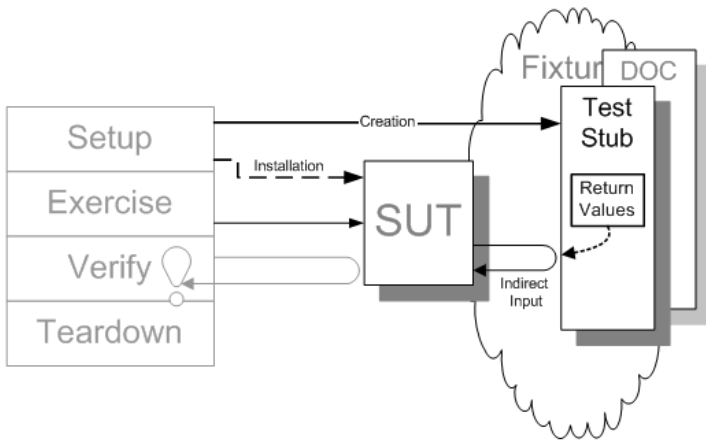
\includegraphics[width=0.6\textwidth]{stub.png}
            \attribution{http://xunitpatterns.com}
        \end{center}
    \end{frame}

    \begin{frame}{Spies}
        \begin{itemize}
            \item Запуск теста, затем проверка условий и ограничений
        \end{itemize}
        \begin{center}
            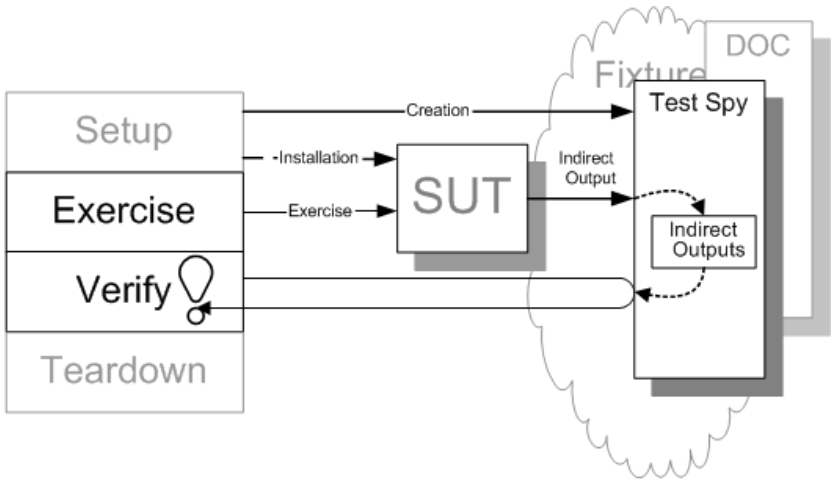
\includegraphics[width=0.6\textwidth]{spy.png}
            \attribution{http://xunitpatterns.com}
        \end{center}
    \end{frame}

    \begin{frame}{Mocks}
        \begin{itemize}
            \item Конфигурирование объекта перед запуском теста
        \end{itemize}
        \begin{center}
            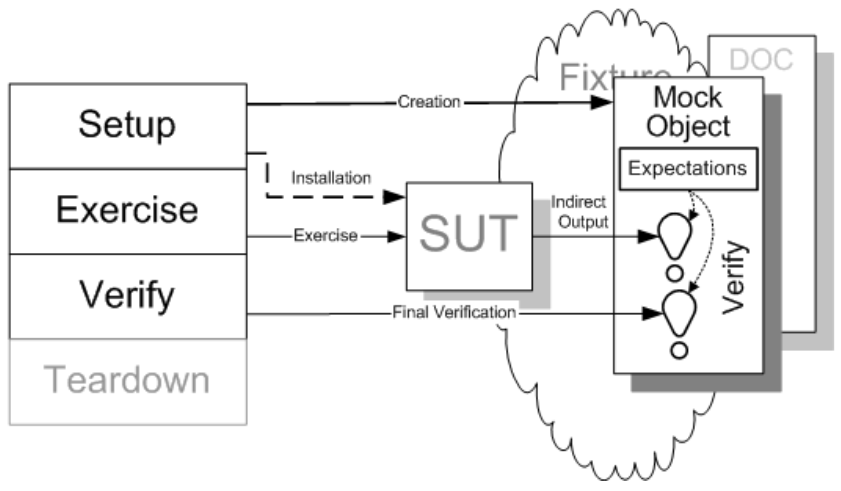
\includegraphics[width=0.6\textwidth]{mock.png}
            \attribution{http://xunitpatterns.com}
        \end{center}
    \end{frame}

    \section{Библиотеки}

    \begin{frame}{Библиотеки}
        \begin{itemize}
            \item Moq (\url{https://github.com/devlooped/moq}) --- стандарт де-факто для моков в тестах на .NET
            \item NSubstitute (\url{https://nsubstitute.github.io/}) --- несколько более \enquote{чистый} синтаксис
            \item FakeItEasy (\url{https://fakeiteasy.github.io/}) --- достойная альтернатива, с местами более аккуратным, а местами более громоздким синтаксисом
        \end{itemize}
    \end{frame}

    \begin{frame}[fragile]{Пример}
        \framesubtitle{Moq}
        \begin{minted}{csharp}
/// Arrange
var mock = new Mock<ILoveThisLibrary>();
mock.Setup(library => library.DownloadExists("2.0.0.0"))
    .Returns(true);
ILoveThisLibrary lovable = mock.Object;

/// Act
bool download = lovable.DownloadExists("2.0.0.0");

// Assert
mock.Verify(library 
    => library.DownloadExists("2.0.0.0"), Times.AtMostOnce());
        \end{minted}
        \attribution{\url{https://github.com/devlooped/moq} (слегка адаптировано)}
    \end{frame}

    \begin{frame}[fragile]{Более жизненный пример (1)}
        \framesubtitle{Moq}
        \begin{small}
            \begin{minted}{csharp}
public class System(IDependency dependency)
{
    public int DoSomething(int x)
        => dependency.ImportantMethod(x);
}

public interface IDependency
{
    int ImportantMethod(int importantParameter);
}

public class Dependency: IDependency
{
    public int ImportantMethod(int importantParameter)
        => importantParameter + 1;
}
            \end{minted}
        \end{small}
    \end{frame}

    \begin{frame}[fragile]{Более жизненный пример (2)}
        \framesubtitle{Moq}
        \begin{small}
            \begin{minted}{csharp}
[Test]
public void TestWithMocks()
{
    var dependencyMock = new Mock<IDependency>();
    dependencyMock.Setup(dependency => dependency.ImportantMethod(1))
        .Returns(2);
    
    var system = new System(dependencyMock.Object);

    var result = system.DoSomething(1);

    Assert.That(result, Is.EqualTo(2));
    dependencyMock.Verify(dependency => dependency.ImportantMethod(1), 
        Times.Exactly(1));
}
            \end{minted}
        \end{small}
    \end{frame}

    \section{Задача на остаток пары}

    \begin{frame}{Задача}
        \begin{itemize}
            \item Вспомнить домашнее задание про стековый калькулятор
            \item Переделать стеки так, чтобы они были генериками
            \item Написать тесты для калькулятора, изолированные от реализации стеков
        \end{itemize}
    \end{frame}

\end{document}
